\section{A general overview}

\begin{frame}
  \frametitle{Summary}
  \tableofcontents[currentsection]
\end{frame}

\subsection{Where does it come from?}

\begin{frame}
  \frametitle{The nature}
  \begin{block}{Natural Selection}
    \begin{itemize}
    \item Darwin\cite{darwin.1840.origin.of.species} introduces
      Natural selection.
    \item It implies several conditions:
      \begin{itemize}
      \item Reproduction of individuals in the population.
      \item Variation that affects the likelihood of survival of
        individuals.
      \item Heredity in reproduction.
      \end{itemize}
    \end{itemize}
  \end{block}

  \begin{block}{Sexual/Asexual?}
    \begin{itemize}
    \item Asexual reproduction is based on cloning, and
      eventually mutation.
    \item Sexual is based on crossover.
    \end{itemize}
  \end{block}
\end{frame}

\begin{frame}
  \frametitle{Link with Genetic Programming?}
  \begin{block}{On the idea}
    \begin{itemize}
    \item Evolve a population to solve a problem.
    \item The population could be a lot of things(programs, parameters\dots).
    \end{itemize}
  \end{block}

  \begin{block}{On the way its done}
    \begin{itemize}
    \item Create the population,
    \item Keep only the best ones,
    \item Make them create a new generation,
    \item And so on until the population solves the problem.
    \end{itemize}
  \end{block}
\end{frame}

\begin{frame}
  \frametitle{A basis graphical overview}
  \begin{center}
    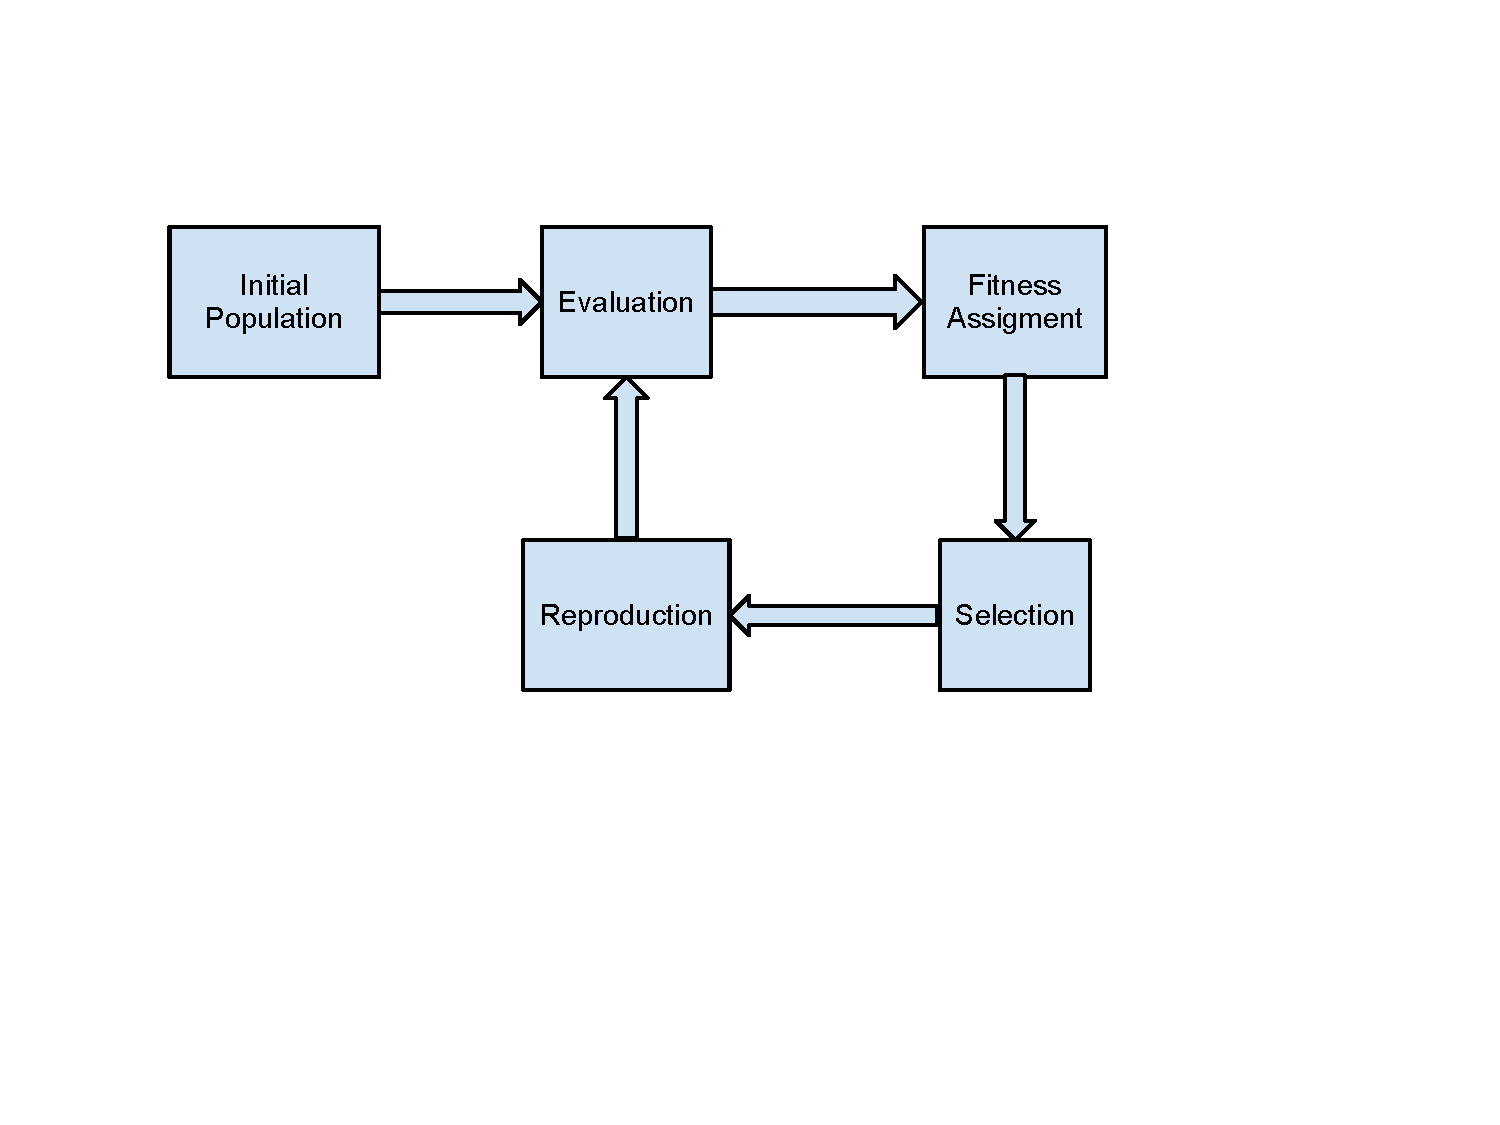
\includegraphics[scale=0.5]{img/cycle}
  \end{center}
\end{frame}

\subsection{When to use Evolutionary Algorithm?}

\begin{frame}
  \frametitle{When to use Evolutionary Algorithm?}
  \begin{block}{When...}
    \begin{itemize}
    \item We can't find a solution with classical computations,
    \item We are able to find a way to evaluate an individual.
    \end{itemize}
  \end{block}

  \begin{block}{Examples}
    \begin{itemize}
    \item Prisoner's dilemma\cite{axelrod1991},
    \item Intrusion detection in a system\cite{crosby1995},
    \item Autoparallelization\cite{walsh1996}.
    \end{itemize}
  \end{block}
\end{frame}

\subsection{Definitions}

\begin{frame}
  \frametitle{EA, GA, GP, ES... ???}
  \begin{block}{In the literature}
    \begin{itemize}
    \item When you are looking for genetic programming, you'll find a
      lot of different things.
    \item In this talk, we consider Evolutionary Algorithm as an
      umbrella term to represent techniques which use evolution.
    \end{itemize}
\end{block}

  \begin{center}
    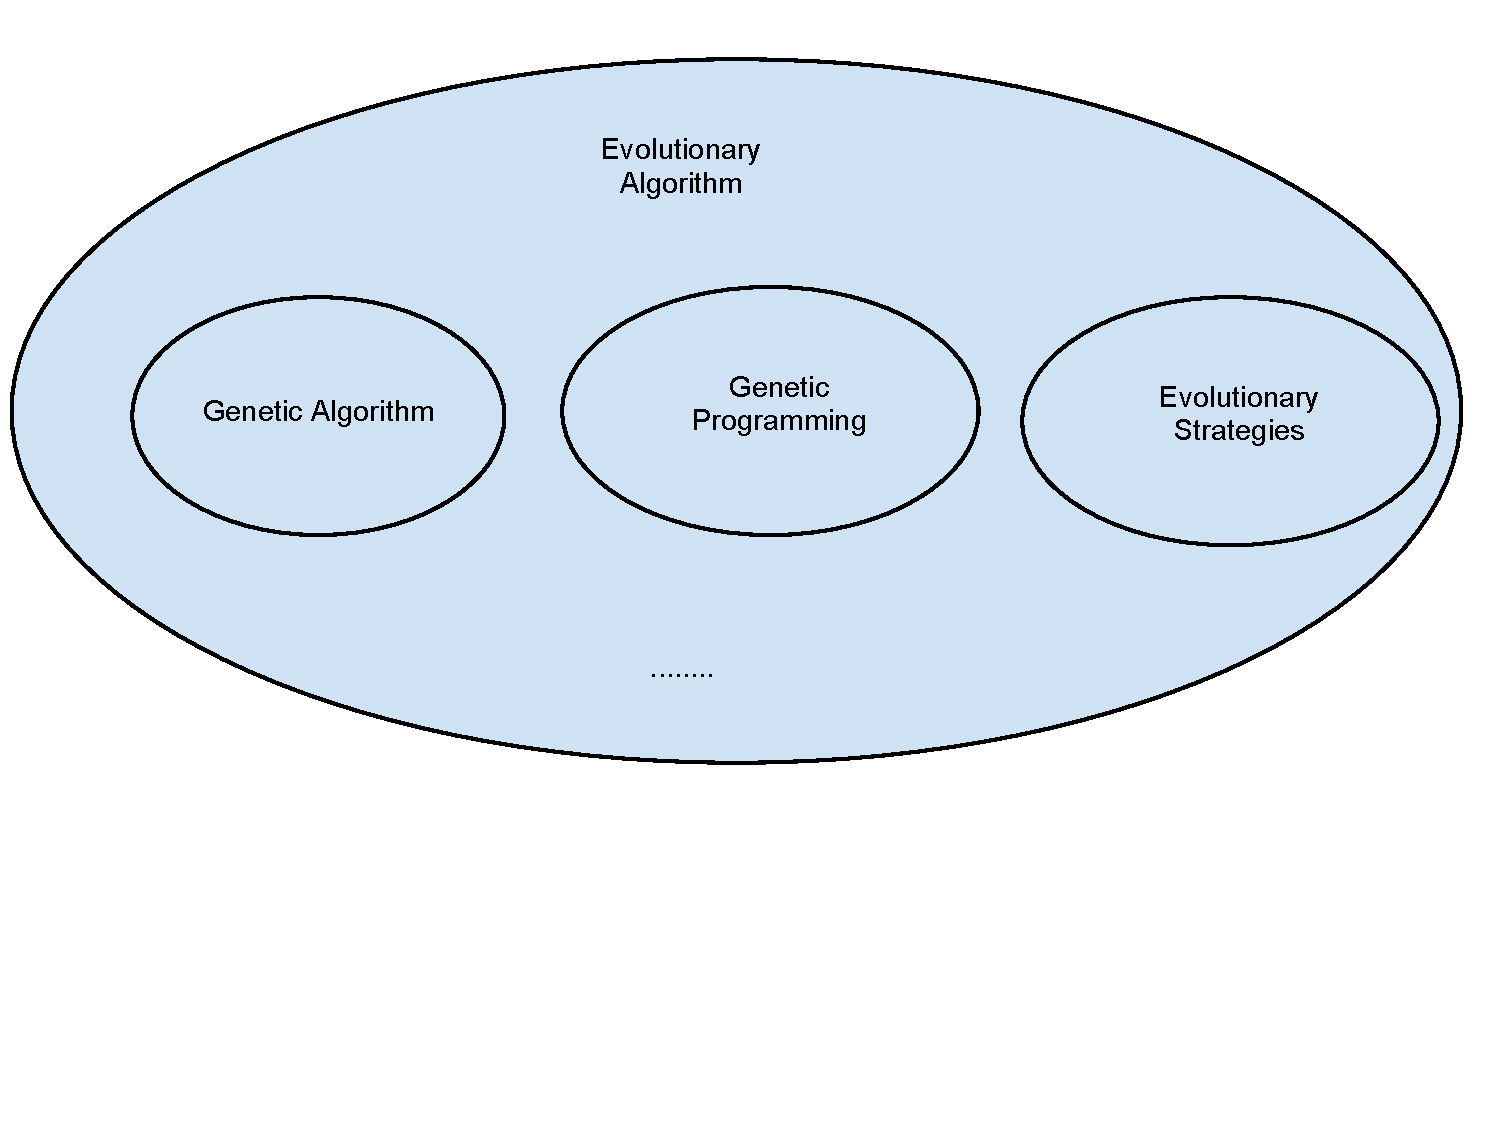
\includegraphics[scale=0.4]{img/ea}
  \end{center}
\end{frame}

\begin{frame}
  \frametitle{Genetic Algorithms}
  \begin{block}{History}
    \begin{itemize}
    \item Developed by Holland\cite{holland1992}.
    \item The original GA uses:
      \begin{itemize}
        \item fixed-length binary representation.
        \item Crossover a lot.
      \end{itemize}
    \item This model has been extended, now GA uses an alphabet (like DNA).
    \item We'll let the theoretical development for the second part.
      %% In this phrase, I mean Pierre, you have to explain the GA 1-point
      %% crossover (GP An introduction p96) and the schemata.
    \end{itemize}
  \end{block}
\end{frame}

\begin{frame}{Genetic Algorithms (cont.)}
  \begin{algorithm}[H]
    \caption{Genetic Algorithm}
    \begin{algorithmic}
      \State t := 0
      \State initPopulation P(t)
      \State evaluate P(t)
      \While {not done}
        \State ++t
        \State P' := selectParents P(t)
        \Comment{Crossover}
        \State recombine P'(t)
        \State mutate P'(t)
        \State evaluate P'(t)
        \State P := survive P', P(t)
      \EndWhile
    \end{algorithmic}
  \end{algorithm}
\end{frame}

\begin{frame}
  \frametitle{Evolutionary Strategies}
  \begin{block}{History}
    \begin{itemize}
    \item Idea started in 1960.
    \item Defined by Rechenberg\cite{Rechenberg.1975} and Schwefel\cite{Schwefel.1981}.
    \end{itemize}
  \end{block}

  \begin{block}{Characteristics}
    \begin{itemize}
    \item Only mutation.
    \item In the selection: each generation is smaller than the
      precedent.
    \end{itemize}
  \end{block}
\end{frame}


\begin{frame}
  \frametitle{Evolutionary Programming}
  \begin{block}{History}
    \begin{itemize}
      \item Created in 1966, by Fogel, Owens, and Walsh\cite{fogel1966}.
    \end{itemize}
  \end{block}

  \begin{block}{Characteristics}
    \begin{itemize}
    \item Works on Finite-State Machine.
    \item Can modify: initial state, number of states, transition\dots
    \item Mutation decreases as the optimal fitness approaches.
    \end{itemize}
  \end{block}
\end{frame}


\begin{frame}
  \frametitle{Genetic Programming}
  \begin{block}{History}
    \begin{itemize}
    \item Works on program instead of parameters.
    \item Introduced by Koza\cite{Koza92}.
    \item Works on parse-tree.
    \end{itemize}
  \end{block}

  \begin{block}{Characteristics}
    \begin{itemize}
    \item Many people use LISP.
    \item Assembly languages are also used.
    \item Example: can find the function $x^2/2$.
    \end{itemize}
  \end{block}
\end{frame}

\subsection{Genetic Operators}

\begin{frame}
  \frametitle{Genetic Operators}
  \begin{block}{What is this?}
    \begin{itemize}
    \item The initial population generally has a very low fitness.
    \item Genetic operators make them evolves.
    \end{itemize}
  \end{block}

  \begin{block}{Who are they?}
    \begin{description}
    \item[Crossover] Create new individuals by mixing.
    \item[Mutation] Create new individuals by random alteration.
    \item[Reproduction] Change the population.
    \end{description}
  \end{block}

\end{frame}

\begin{frame}
  \frametitle{Crossover}
  \begin{block}{The concept}
    \begin{itemize}
    \item Mix the genome.
    \item Create new elements.
    \item There are a lot of different techniques.
    \end{itemize}
  \end{block}

  \begin{block}{Tree-based Crossover}
    \begin{itemize}
    \item Select randomly two nodes in two trees, and exchange their
      child.
    \end{itemize}
  \end{block}
\end{frame}


\begin{frame}
  \frametitle{Crossover (cont.) - Linear crossover}
  \begin{figure}[ht]
    \centering
    \visible<1-3>{
      \subfigure{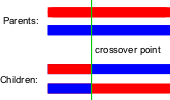
\includegraphics[width=4.5cm]{img/SinglePointCrossover}}
    }
    \visible<2-3>{
    \subfigure{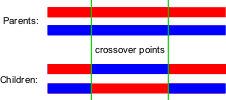
\includegraphics[width=4.5cm]{img/TwoPointCrossover}}
    }
    \visible<3>{
    \subfigure{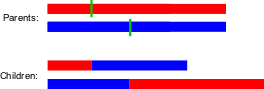
\includegraphics[width=4.5cm]{img/CutSpliceCrossover}}
  }
  \end{figure}
\end{frame}

\begin{frame}
  \frametitle{Mutation}
  \begin{block}{Concept}
    \begin{itemize}
    \item Operate on only one individual.
    \item Generally after the crossover.
    \item Low probability.
    \end{itemize}
  \end{block}

  \begin{block}{On tree structures}
    \begin{itemize}
    \item Take randomly a node, and replace its children by a new subtree
      randomly created.
    \item This subtree respects the limitation (size, depth\dots) on
      the tree.
    \end{itemize}
  \end{block}
\end{frame}

\begin{frame}
  \frametitle{Mutation (cont.)}
  \begin{block}{On linear structures}
    \begin{itemize}
    \item Take an element randomly.
    \item Apply one or more changes.
    \end{itemize}
  \end{block}

  \begin{block}{Example}
    \begin{itemize}
    \item Suppose we are in GP, ``$r_0 = r_1 + r_2$'' could become:
      \begin{itemize}
      \item $r_1 = r_1 + r_2$
      \item $r_0 = r_1 - r_2$
      \item $r_0 = r_0 + r_0$
      \item \dots
      \end{itemize}
    \end{itemize}
  \end{block}
\end{frame}

\begin{frame}
  \frametitle{Reproduction}
  \begin{block}{Concept}
    \begin{itemize}
    \item If an individual is selected, it is copied.
    \item Two versions of the same individual (unless we chose to kill
      the parents).
    \end{itemize}
  \end{block}
\end{frame}

\begin{frame}
  \frametitle{Fitness}
  \begin{block}{Concept}
    \begin{itemize}
    \item This is the function which allows to classify an individual.
    \item There is a lot of way to consider this function\dots
    \end{itemize}
  \end{block}

  \begin{block}{Examples}
    \begin{itemize}
    \item The number of matching pixels in an image matching application.
    \item The number of wall hits for a robot controlled by GP and
      learning obstacles avoidance.
    \item The number of correctly classified examples in a
      classification tasks.
    \item The money won by a GP-controlled agent in a betting game.
    \item \dots
    \end{itemize}
  \end{block}
\end{frame}

\begin{frame}
  \frametitle{The Selection Algorithm}
  \begin{block}{Concept}
    \begin{itemize}
    \item The way we select individuals.
    \item There is a lot of way.
    \end{itemize}
  \end{block}

  \begin{block}{Fitness Proposal Selection}
    \begin{itemize}
    \item Used for GA-type algorithms.
    \item Introduced by Holland\cite{holland1992}.
    \item $p_i = f_i / \sum_{j}f_j$
    \end{itemize}
  \end{block}
\end{frame}

\begin{frame}
  \frametitle{The Selection Algorithm (cont.)}
  \begin{block}{Truncation}
    \begin{itemize}
    \item Used for ES-type algorithms,
    \item Introduced by Schwefel\cite{schwefel1995},
    \item Coma-evolution: All parents died before selection,
    \item Plus-evolution: Everyone are considered for selection,
    \item We take only the $\mu$ best individuals.
    \end{itemize}
  \end{block}

  \begin{block}{Ranking}
    \begin{itemize}
    \item Based on the fitness order.
    \item Two kind on ranking are (mainly) used, linear and exponential.
    \end{itemize}
  \end{block}
\end{frame}

\begin{frame}
  \frametitle{The Selection Algorithm (cont.)}
  \begin{block}{Tournament}
    \begin{itemize}
    \item It is a competition in a subset of the population.
    \item Participants are randomly selected.
    \item The size is a parameters of the algorithm, and allow to
      adjust the selection pressure.
    \item The winners of the tournament are selected.
    \item This is a mainstream method for selection.
    \item Easy to parallelize.
    \end{itemize}
  \end{block}

  \begin{block}{Roulette wheel}
    \begin{itemize}
    \item All the population is on a contiguous segment.
    \item The size of an individual segment is proportional to its fitness.
    \item We select N times a random number (N is the size of the
      next generation).
    \item The individual whose segment spans the random number is selected.
    \end{itemize}
  \end{block}
\end{frame}


%%% Local Variables:
%%% mode: latex
%%% mode: flyspell
%%% TeX-master: "../genetic"
%%% ispell-dictionary: "en"
%%% compile-command: "cd .. && make"
%%% End:
